% copyright arturo salinas-aguayo 2025
\documentclass[12pt]{article}

\usepackage{graphicx} \usepackage{subcaption} \usepackage{amsmath}
\usepackage{siunitx} \usepackage{array} \usepackage{amsfonts}
\usepackage{fancyhdr} \usepackage{geometry} \usepackage{circuitikz}
\usepackage{caption} \usepackage{karnaugh-map} \usepackage{bm}
\usepackage{float}

\geometry{letterpaper, margin=1in} \graphicspath{ {../../images/} }

% Header and Footer
\pagestyle{fancy} \fancyhf{} \fancyhead[L]{ECE 3201 - Lab 02: Zener Diode -- Load Line Regulation}
\fancyhead[R]{\thepage} \setlength{\headheight}{15pt}

\author{Arturo Salinas-Aguayo} \title{Lab 02: Zener Diode -- Load Line Regulation}

% theorem set
\newtheorem{example}{Example}
% Example block environment
\newenvironment{examp} {\vspace{0.5cm} \hrule \vspace{0.5cm}
	\begin{example}} {\hrule \vspace{0.5cm}
\end{example}}

\begin{document}
\newcommand{\closure}[2][3]{%
	{}\mkern#1mu\overline{\mkern-#1mu#2}}
\newcommand\ncoverline[1]{\mkern1mu\overline{\mkern-1mu#1\mkern-1mu}\mkern1mu}

% Title Page
\begin{titlepage}
	\centering \vspace*{3cm} \huge\textbf{Lab 02: Zener Diode -- Load Line Regulation}\\

	\vspace{5cm} \Large\textbf{Arturo Salinas-Aguayo}\\
	\normalsize ECE 3201 Electronic Circuit Design and Analysis\\
	Dr. Mehdi Anwar\\
	Electrical and Computer Engineering Department\\
	\vfill 
\includegraphics[scale=0.1]{uconnlogo}\\
	College of Engineering, University of Connecticut\\
	\scriptsize{Coded in \LaTeX} \vspace*{1cm}
\end{titlepage}

\tableofcontents

\newpage

\section{Abstract}
This experiment investigates the voltage regulation properties of a Zener diode
in both unloaded and loaded conditions. A 12~V Zener diode was biased through a
series resistor and tested under three configurations: no external load,
a moderate $3~\text{k}\Omega$ load, and a heavy $470~\Omega$ load. Measured
data showed that the Zener maintained approximately 11.5~V under no-load
conditions, with current through the diode increasing slightly as the input
voltage rose. When resistive loads were applied, however, the diode dropped out
of regulation, supplying negligible current and allowing the output voltage to
fall below the nominal breakdown voltage. Simulated results matched closely
with experimental observations, validating the diode model and highlighting the
limitations of Zener regulation when the series resistor cannot support both
the load current and the Zener bias. The experiment demonstrates the importance
of proper resistor sizing in maintaining Zener operation within its breakdown
region.

\newpage
\section{Introduction}
The Zener diode is widely used as a voltage reference and regulator because of
its nearly constant reverse breakdown voltage over a broad range of current.
This lab focuses on exploring the Zener's regulation behavior under different
loading conditions and comparing experimental results with circuit simulations.

\section{Objective}
The objective of this lab is to investigate Zener diode voltage regulation,
demonstrate the impact of load resistance on regulation performance, and compare
measured results to simulated results using a custom diode model.

\section{Theory}
The almost vertical drop of the i-v curve of the Zener diode
in the breakdown region suggests it can be used as a voltage regulator. A
voltage regulator intends to provide a constant DC output voltage, irrespective
of:
\begin{itemize}
  \item \textbf{Load Regulation:} Variation in load current
  \item \textbf{Line Regulation:} Variation in supply voltage
\end{itemize}

For current smaller than the knee current ($-I_{ZK}$), the current remains
almost constant. $V_{Z}$ and $I_{ZT}$ are test parameters provided by the
manufacturer. As the current deviates from the test current $I_{ZT}$, the
voltage also changes, resulting in a small resistance,
$r_{Z} = \Delta V / \Delta I$. $r_{Z}$ is typically in the range of a few ohms
to tens of ohms; the lower the value of $r_{Z}$, the more stable the performance
of the Zener diode.
\[
\Delta V = \Delta I \cdot r_{Z}
\]

\begin{figure}[H]
  \centering
  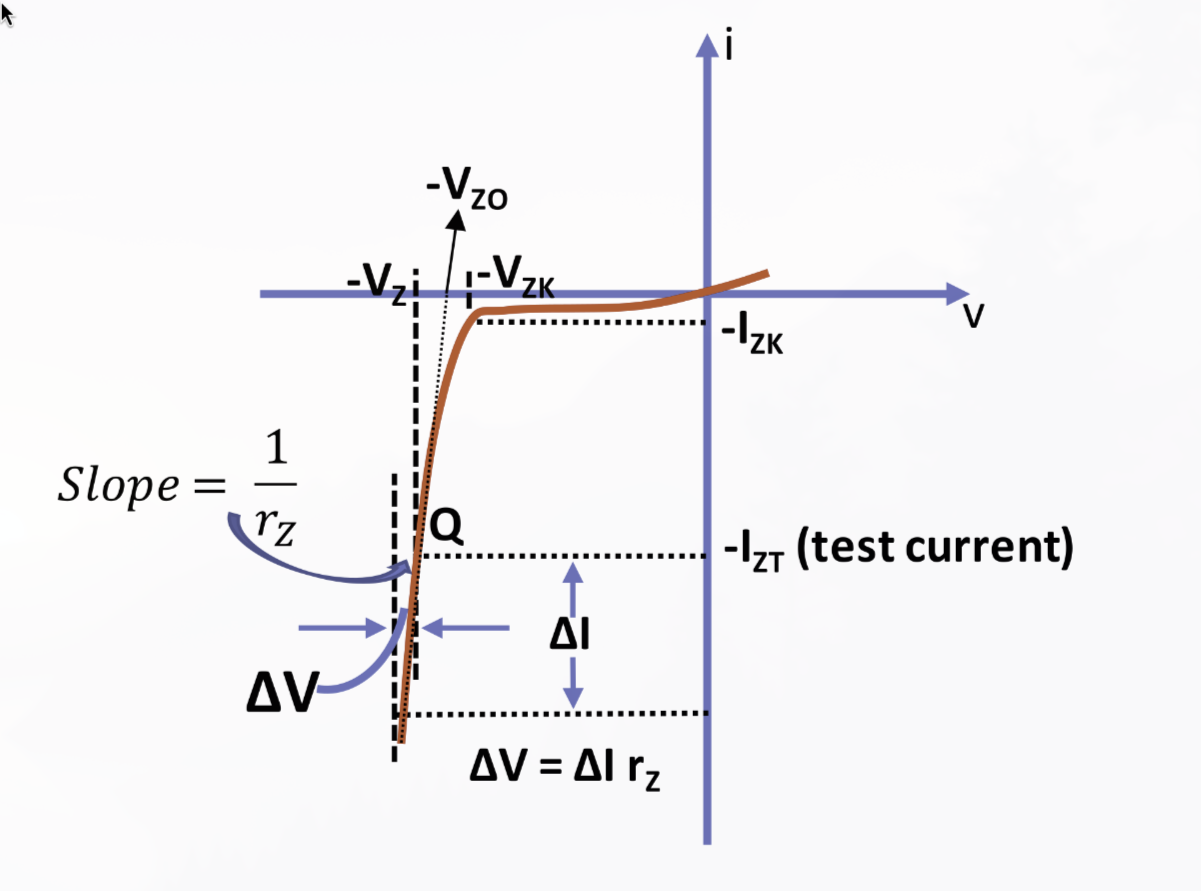
\includegraphics[width=0.5\textwidth]{lab02/curve.png}
  \caption{Zener diode i-v characteristics}
  \label{fig:zener_iv}
\end{figure}

The almost linear i-v characteristic of the Zener diode allows it to be modeled
as shown in Figure~\ref{fig:zener_model}, with a constant voltage source
($V_{ZO}$) in series with $r_{Z}$. From this representation:
\[
V_{Z} = V_{ZO} + r_{Z} I_{Z}, \quad \text{for } I_{Z} > I_{ZK}, \, V_{Z} > V_{ZO}
\]

\begin{figure}[H]
  \centering
  \begin{circuitikz}[american]
    \draw (0,0) to[battery1, l=$V_{ZO}$] (2,0)
          to[R=$r_Z$] (4,0) -- (5,0) node[right] {$V_Z$};
  \end{circuitikz}
  \caption{Small-signal Zener diode equivalent circuit}
  \label{fig:zener_model}
\end{figure}

\section{Experimental Procedures}
The following circuits were utilized in order to determine the characteristics
of the Zener diode in an introductory fashion.
\begin{figure}[H]
  \centering
  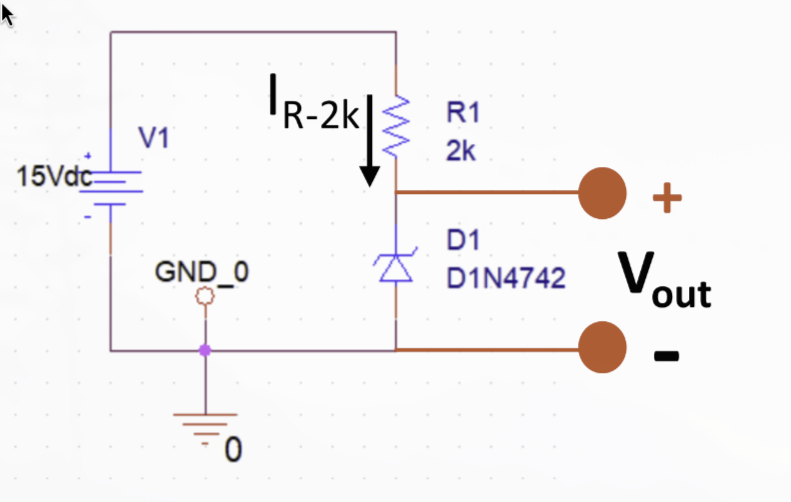
\includegraphics[width=0.8\textwidth]{lab02/noload.png}
  \caption{Circuit 1 -- No Load}
\end{figure}
\begin{figure}[H]
  \centering
  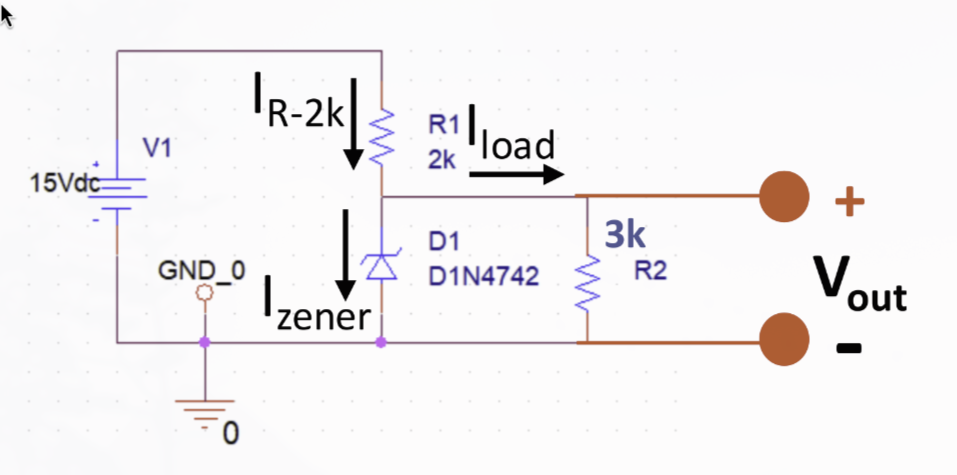
\includegraphics[width=0.8\textwidth]{lab02/load.png}
  \caption{Circuit 2/3 -- With Resistive Loads}
\end{figure}

\begin{table}[H]
  \caption{Reistor Values}
  \begin{center}
    \begin{tabular}[c]{|c|c|}
      \hline
      \multicolumn{1}{|c|}{Resistor} &
      \multicolumn{1}{|c|}{Measured Value} \\
      \hline
      $2K\Omega$ & $2.00K\Omega$ \\
      $3K\Omega$ & $3.01K\Omega$ \\
      $0.47K\Omega$ & $0.470K\Omega$ \\
      \hline
    \end{tabular}
  \end{center}
\end{table}


\section{Results}
\subsection{Circuit 1 - No Load Condition}
\begin{table}[H]
  \caption{Circuit 1 - No Load}\label{tab:noload}
  \begin{center}
    \begin{tabular}[c]{|l|l|l|l|}
      \hline
      \multicolumn{1}{|c|}{\textbf{$V_{IN}$}} &
      \multicolumn{1}{|c|}{\textbf{14V}} &
      \multicolumn{1}{|c|}{\textbf{15V}} &
      \multicolumn{1}{|c|}{\textbf{16V}} \\
      \hline
      \textbf{$V_{2K\Omega}$} & 2.54V & 3.53V & 4.52V  \\
      \textbf{$V_{Zener}$} & 11.48V & 11.49V & 11.50V \\
      \textbf{$I_{Zener}$} & 1.28mA & 1.77mA & 2.27mA \\
      \hline
    \end{tabular}
  \end{center}
\end{table}

\subsection{Circuit 2 - $3K\Omega$ Load}
\begin{table}[H]
  \caption{Circuit 2 - 3K Load}\label{tab:3kload}
  \begin{center}
    \begin{tabular}[c]{|l|l|l|l|}
      \hline
      \multicolumn{1}{|c|}{\textbf{$V_{IN}$}} &
      \multicolumn{1}{|c|}{\textbf{14V}} &
      \multicolumn{1}{|c|}{\textbf{15V}} &
      \multicolumn{1}{|c|}{\textbf{16V}} \\
      \hline
      \textbf{$V_{2K\Omega}$} & 5.58V & 5.98V & 6.38V  \\
      \textbf{$V_{Zener}$} & 8.43V & 9.03V & 9.63V \\
      \textbf{$I_{R2K\Omega}$} & 2.80mA & 3.00mA & 3.20mA \\
      \textbf{$I_{load}$} & 2.80mA & 3.00mA & 3.20mA \\
      \textbf{$I_{Zener}$} & $0.2\,\mu\text{A}$ & $0.2\,\mu\text{A}$ & $0.2\,\mu\text{A}$ \\
      \hline
    \end{tabular}
  \end{center}
\end{table}

\subsection{Circuit 3 - $0.47K\Omega$ Load}
\begin{table}[H]
  \caption{Circuit 3 - 0.47K Load}\label{tab:.47kload}
  \begin{center}
    \begin{tabular}[c]{|l|l|l|l|}
      \hline
      \multicolumn{1}{|c|}{\textbf{$V_{IN}$}} &
      \multicolumn{1}{|c|}{\textbf{14V}} &
      \multicolumn{1}{|c|}{\textbf{15V}} &
      \multicolumn{1}{|c|}{\textbf{16V}} \\
      \hline
      \textbf{$V_{2K\Omega}$} & 11.33V & 12.07V & 12.94V  \\
      \textbf{$V_{Zener}$} & 2.68V & 2.87V & 3.07V \\
      \textbf{$I_{R2K\Omega}$} & 5.70mA & 6.10mA & 6.52mA \\
      \textbf{$I_{load}$} & 5.70mA & 6.10mA & 6.52mA \\
      \textbf{$I_{Zener}$} & $0.2\,\mu\text{A}$ & $0.2\,\mu\text{A}$ & $0.2\,\mu\text{A}$ \\
      \hline
    \end{tabular}
  \end{center}
\end{table}

\subsection{Line Regulation Analysis}
The variation in Zener voltage with respect to supply voltage was measured
experimentally for three different load conditions:
\begin{itemize}
  \item \textbf{No Load:} $V_{IN}$: 14$\to$16~V, $V_{Z}$: 11.48$\to$11.50~V.\\
  Slope $\Delta V_Z / \Delta V_{IN} = 0.01~\text{V/V}$ (10~mV per volt).\\
  Percentage change over the span: $(0.02/11.48)\times 100\% \approx 0.17\%$.
  \item \textbf{3 k$\Omega$ Load:} $V_{Z}$: 8.43$\to$9.63~V for the same input change.\\
  Slope $= 0.60~\text{V/V}$ (poor regulation; Zener off).
  \item \textbf{470 $\Omega$ Load:} $V_{Z}$: 2.68$\to$3.07~V.\\
  Slope $= 0.20~\text{V/V}$ (dominated by divider action; Zener off).
\end{itemize}

\subsection{Load Regulation Analysis}
As load current increased (no load $\to$ $3~\text{k}\Omega$ $\to$ $470~\Omega$),
the Zener voltage fell from $\sim$11.5~V to $\sim$9~V and then to $\sim$3~V.
This shows that the series resistor must provide enough current to satisfy both
the load and a minimum Zener current (above $I_{ZK}$) or regulation is lost.

\subsection{Derived Device Parameters}
From the no-load measurements around 14--16~V:
\[
\Delta V_Z \approx 0.02~\text{V},\quad \Delta I_Z \approx 2.27-1.28=0.99~\text{mA}
\]
\[
\Rightarrow \; r_Z \approx \frac{\Delta V_Z}{\Delta I_Z} \approx
\frac{0.02}{0.00099} \approx 20~\Omega
\]
This is larger than the datasheet $r_{Z T}\approx 9~\Omega$ at $I_{Z T}=21$~mA,
as expected, since our operating current (1--2~mA) is well below the test
current and the Zener slope is steeper (higher $r_Z$) at lower currents.

\paragraph{Voltage Variation vs.\ $V_{IN}$ (measured)}
\begin{itemize}
  \item No load: $\Delta V_Z/\Delta V_{IN}=0.01~\text{V/V}$ (\SI{10}{mV/V}).
  \item $3~\text{k}\Omega$ load: $\Delta V_Z/\Delta V_{IN}=0.60~\text{V/V}$.
  \item $470~\Omega$ load: $\Delta V_Z/\Delta V_{IN}=0.20~\text{V/V}$.
\end{itemize}

\paragraph{Zener Current Variation vs.\ $V_{IN}$ (measured)}
\begin{itemize}
  \item No load: $I_Z$:\;1.28$\to$2.27~mA over $\Delta V_{IN}=2$~V
  $\Rightarrow \Delta I_Z/\Delta V_{IN}\approx 0.99/2=\SI{0.495}{mA/V}$.
  \item $3~\text{k}\Omega$ load: $I_Z \approx \SI{0.2}{\micro A}$ (constant) $\Rightarrow$ slope $\approx 0$.
  \item $470~\Omega$ load: $I_Z \approx \SI{0.2}{\micro A}$ (constant) $\Rightarrow$ slope $\approx 0$.
\end{itemize}

\subsection{Simulated Portion}
The following netlist was used to produce the simulated data. For the $3~\text{k}\Omega$
case, set \verb|R2 N002 0 3k|; for the no-load case, omit \verb|R2|.
\begin{verbatim}
* Lab 02 - Zener Diode -- Load Line Regulation
* Arturo Salinas-Aguayo
* 05 September 2025
* @Begin
V1 N001 0 14
D1 0 N002 D1N4742
R1 N001 N002 2k
R2 N002 0 0.47k
.dc v1 14 16 .5
.model D1N4742 D( BV=12  IBV=0.021  NBV=7.31  RS=0.5
+ IS=1e-9  N=1.5  CJO=80p  VJ=0.7  M=0.33  TT=50n )
.end
* @End
\end{verbatim}
\begin{itemize}
  \item Instantiates a DC source, Zener diode (custom model), and resistors.
  \item Performs a DC sweep in \SI{0.5}{V} steps from \SI{14}{V} to \SI{16}{V}.
  \item Note: Negative simulated $I_{Zener}$ values arise from the standard device current reference direction (from anode to cathode).
\end{itemize}

\subsection{Simulation Data - Circuit 1 -- No Load}
\begin{table}[H]
  \caption{Simulated Circuit 1 - No Load}\label{tab:simnoload}
  \begin{center}
    \begin{tabular}[c]{|l|l|l|l|}
      \hline
      \multicolumn{1}{|c|}{\textbf{$V_{IN}$}} &
      \multicolumn{1}{|c|}{\textbf{14V}} &
      \multicolumn{1}{|c|}{\textbf{15V}} &
      \multicolumn{1}{|c|}{\textbf{16V}} \\
      \hline
      \textbf{$V_{Zener}$} & 11.469V & 11.529V & 11.576V \\
      \textbf{$I_{Zener}$} & -1.265mA & -1.735mA & -2.212mA \\
      \hline
    \end{tabular}
  \end{center}
\end{table}

\subsection{Simulation Data - Circuit 2 -- $3K\Omega$ Load}
\begin{table}[H]
  \caption{Simulated Circuit 2 - $3K\Omega$ Load}\label{tab:sim3kload}
  \begin{center}
    \begin{tabular}[c]{|l|l|l|l|}
      \hline
      \multicolumn{1}{|c|}{\textbf{$V_{IN}$}} &
      \multicolumn{1}{|c|}{\textbf{14V}} &
      \multicolumn{1}{|c|}{\textbf{15V}} &
      \multicolumn{1}{|c|}{\textbf{16V}} \\
      \hline
      \textbf{$V_{Zener}$} & 8.399V & 8.999V & 9.599V \\
      \textbf{$I_{Zener}$} & -1.121nA & -3.708nA & -65.472nA \\
      \hline
    \end{tabular}
  \end{center}
\end{table}

\subsection{Simulation Data - Circuit 3 -- $0.47K\Omega$ Load}
\begin{table}[H]
  \caption{Simulated Circuit 3 - $0.47K\Omega$ Load}\label{tab:sim47kload}
  \begin{center}
    \begin{tabular}[c]{|l|l|l|l|}
      \hline
      \multicolumn{1}{|c|}{\textbf{$V_{IN}$}} &
      \multicolumn{1}{|c|}{\textbf{14V}} &
      \multicolumn{1}{|c|}{\textbf{15V}} &
      \multicolumn{1}{|c|}{\textbf{16V}} \\
      \hline
      \textbf{$V_{Zener}$} & 2.664V & 2.854V & 3.044V \\
      \textbf{$I_{Zener}$} & -1.00nA & -1.00nA & -1.00nA \\
      \hline
    \end{tabular}
  \end{center}
\end{table}

\subsection{Summary}
The experimental data confirm the theoretical behavior: under no load, the Zener
provides excellent line regulation, but with significant loading the diode drops
out of conduction. Proper resistor sizing and supply design are therefore
critical to maintain regulation.

\section{Conclusion}
The results confirm that Zener diodes regulate effectively only when biased
with sufficient current. In the no-load condition, the Zener voltage remained
stable near 11.5~V, with the diode absorbing excess current from the series
resistor. Under a $3~\text{k}\Omega$ load, however, nearly all current was
diverted to the load, causing the Zener to conduct almost no current and the
regulated voltage to drop to the 8--9~V range. With a heavier $470~\Omega$ load,
the diode was fully out of regulation, and the voltage collapsed to 2--3~V.
Simulation data reproduced these behaviors, reinforcing the experimental
observations. The key design insight is that the series resistor and supply
voltage must be chosen such that the diode maintains a bias current above its
minimum value even under maximum load. Without this condition, the Zener cannot
act as a reliable voltage regulator.

\end{document}
